\chapter{Introduction}

Radars have several highly attractive properties: commonly, they are active systems independent of lighting conditions, are very fast and have high precision. Furthermore, implemented at millimeter-wave wavelengths, radar sensors can be designed as low-power devices with no moving parts in a favorable form factor \citep{lien_gillian_karagozler_amihood_schwesig_olson_raja_poupyrev_2016}.

Radar technology has been around since the 1930s \citep{watson-watt_1945}, and has since developed into a well-established field of engineering. Although the typical use case in radio frequency (\gls{rf}) radars regard detection and tracking of large objects at far distances, such as for air and marine monitoring, new areas of applications have emerged during recent years, posing very different engineering challenges. Some of these are outlined in \citep{amin_2017}, where close-range radars are used for applications such as vital signs monitoring \citep{kuo_lin_yu_lo_lyu_chou_chuang_2016}, gesture recognition \citep{lien_gillian_karagozler_amihood_schwesig_olson_raja_poupyrev_2016} and tumor imaging \citep{klemm_gibbins_leendertz_horseman_preece_benjamin_craddock_2011}, to name a few. Furthermore, millimeter-wave radars have lately become more inexpensive, largely due to their widespread adoption in the automotive industry \citep{frenzel_2018}, making such devices an attractive option in a wide range of low-cost applications. %Alongside the miniaturization of radar systems a trend in data science has emerged; the movement towards machine learning centric methods. This transition, spanned over multiple decades, has placed machine learning as an increasingly popular choice for data analysis. Machine learning algorithms encompass a very large set of algorithms, but fundamentally utilize various statistical techniques in order to allow computer systems to progressively improve performance \citep{a_smola_svn_vishwanathan_2010}. Data scientists have found machine learning, which forms a subclass of aritficial intelligence, particularly practical for data that lack an easily predictable structure.

In this work, we investigate whether millimeter-wave radar can be used for surface classification of rough surfaces. Two broad antenna beams illuminate a target scene, and using a feature extraction procedure and machine learning techniques, the returning echoes are analyzed to determine the surface type. This work focuses on the use case of determining if a surface is grassy or not, but could be extended to other surface types.  

\section{Motivation and Previous Work}

Autonomous robots have found increasing use in numerous devices, from helping customers navigate stores \citep{mcsweeney_2018} to keeping floors clean \citep{sanfacon_2017} and mowing lawns \citep{udelhofen_2018}. A common challenge in such systems is keeping the robot in bounds. This commonly means for the robot to be aware where on a two-dimensional map it is currently located. In certain applications staying in bounds rather involves remaining on a set of allowed surface types, such as for autonomous robot lawn mowers remaining only on areas covered in grass. In such devices one may be content with knowing that the robot roams around remaining on its designated surface type rather than having knowledge of its exact position, and hence a surface classification method would be of great use. 

Surface classification can also be used in autonomous devices as a supporting system. A robot vacuum cleaner could for instance make use of such a system in numerous ways, such as for avoiding liquid spills or using surface-dependent cleaning programs. One could easily imagine other use cases where knowledge of which surface type an autonomous device is on would be a great convenience.

The task of surface classification can be achieved in many ways. Taking inspiration from the recent advances in computer vision \citep{liu_chen_fieguth_zhao_chellappa_pietikainen_2018}, surfaces could be examined optically and separated by their differences in texture - their spatial organization of image elements \citep{do_vetterli_2002}. Another method is employing direct surface contact. In \citep{giguere_dudek_2011}, surface identification was performed for low velocity mobile robots using a small metallic rod with an attached accelerometer, capturing motion signatures when traversing a surface. Researches, perhaps motivated by experiments showing bats capable of distinguishing surface roughness by using their echolocation \citep{schmidt_1988}, have also experimented with ultrasonic methods for use in road condition monitoring \citep{bystrov_2016}, \citep{mckerrow_kristiansen_2006}. 
%In order to distinguish one surface type from another some feature of the surface at hand must somehow be captured and analyzed. This very general problem statement can and has been approached from many different angles.

% Shorten down from here!

%Taking inspiration from the recent advances in computer vision, one may be tempted to use cameras for visual inspection of the surface at hand. Computer vision has indeed attracted extensive research over the past few decades with impressive results \citep{liu_chen_fieguth_zhao_chellappa_pietiaäinen_2018}. In a computer vision framework, images of different surfaces can be separated by their differences in \emph{texture} - their spatial organization of basic elements. Such fundamental microstructures obey some kind of statistical properties which can be percepted by for instance a convolutional neural network. Effective texture identification of textures in image databases was used in, for example, \citep{do_vetterli_2002} for accuracte classification. 

%Although using computer vision for accurate real time target identification is an attractive option, it is commonly an infeasible option for small devices with limited hardware capabilities. Cameras capture light in the visible frequency spectrum, which inherently renders them sensitive to changes in light conditions. Thus, unless direct illumination of the target surface is used, solutions involving cameras are highly dependent on ambient light. Such a limitation can make cameras impractical for small devices navigating areas with varying lighting.

%The perhaps most immediate way to perform surface identification is through direct contact. In \citep{giguere_dudek_2011}, surface identification for low-velocity mobile robots using a small metallic rod with an attached accelerometer. By capturing accelerometer output induced in the tip of the rod during robot motion identification was possible for a couple of different surface types. While probing may produce appealing results in certain situations, the method is fundamentally based on physical contact with the target. Hence, a probe is more susceptible to damage, can more easily get stuck and is more exposed to detrimental tear over time than its non-interfering counterparts.

% Two chief methods for doing this - Ultrsonic and radar. 
%For surface classification with devices in motion, the seemingly two chief non-contact methods researchers have spent their time on for this application are ultrasonic methods and radar-based methods. These two methods are both noninvasive and have modest power requirements. Furthermore, both are active systems and thus do not need to rely on any ambient signal source. Ultrasonic and radar systems have been tested by researchers for road condition monitoring \citep{bystrov_2016}, \citep{mckerrow_kristiansen_2006}. 

%These two methods primarily utilize the difference in roughness, a geometric characteristic of a surface caused by spatial variations in surface depth. Researchers experimenting with ultrasonic sensors (perhaps motivated by a study proving bats capable of discriminating surfaces with different roughness with their echolocation \citep{schmidt_1988}) have found some degree of success. In \citep{politis_probert_1999} angled ultrasonic sensors were used to measure roughness. By comparing the distribution of energy between specular (i.e. mirror-like) and diffuse componenets of ultrasonic echo they were able to distinguish between six different surface types, and modeling the floor as having a random structure on the form of a Gaussian distribution around the surface plane creating. Using this method the researchers were able to generate predictions on a sample-by-sample basis, not taking the temporal dimension into account.
% Work with the last part here - radar applications/radarCat etc. We wish to utilize time-based methods. Would be neat to find radar work doing nearly the same thing. Finally - we are using a single recieving antenna.

In this work, we are interested in distinguishing grass surfaces from non-grass surfaces using millimeter-wave radar. The application most closely resembling this objective is perhaps the use of millimeter-wave radar for road condition monitoring, where one attempts to determine the state of a road for safety and driver assistance purposes.

Several methods involving measuring polarizations have been proposed for this purpose. In \citep{finkele_schreck_wanielik_1995}, an array of radar transmitters and receivers with different polarities were used sequentially to illuminate the same surface area. Other bistatic setups (configurations with transmitter and receiver spatially separated) for road condition monitoring were considered in \citep{kees_detlefsen_1994} and \citep{finkele_1997}. Monostatic experiments, with transmitting and receiving antenna at the same location, have found varying degrees of success. In \citep{viikari_varpula_kantanen_2008} and \citep{hakli_saily_koivisto_huhtinen_dufva_rautiainen_toivanen_nummila_2013}, a monostatic setup was used to compare returning strengths of differently polarized radar radiation. 

% Work here!
% \citep{fung_pan_1987} - backscattering model, assumes stationary zero mean Gaussian process with some surface correlation function. 


%Backscattering of radiation from random rough surfaces have indeed been studied in several papers. Finding a working model of this is however difficult, as was found in modelling backscattering processes from random rough surfaces, readily showcased in \citep{fung_li_chen_1992}. In \citep{scharf_iberle_mantz_walter_waldschrnidt_2018} simulations and experiments with rough surface backscattering was done by modeling a surfaces topography using a two dimensional autocorrelation function. That paper assumes profiles with moderate slopes and roughness depths and is based on the surface exhibiting a Gaussian height distribution, making it unsuitable for modeling the structures investigated in this paper, other than perhaps gravel. 
These polarization-based methods are founded on measuring the polarization effects of adding a thin layer of ice or water onto a flat asphalt surface. Since the reflectivity of polarized radiation depends both on the polarization and the index of refraction of the reflector one can create a setup founded in well established physics to determine the surface type. These methods rely on illuminating a planar surface, and can thus not effectively be used for the application considered in this report where target surfaces may have large variations in height such as in lawns. In the present case of distinguishing grass we are instead more interested in capturing the \emph{topography} of a surface, not captured as slight differences in polarization.

Backscattering from rough surfaces have been studied in for instance \citep{fung_pan_1987} and \citep{fung_li_chen_1992}, clearly showcasing the difficulties in the modeling of scattering processes from irregular targets. In these papers, a surface is modeled having a Gaussian height distribution with a correlation function determining its shape. Such modeling requires detailed prior knowledge of the surface at hand and does not capture the many complexities arising in real-world surface structures and could hardly be of any great use for this project. In \citep{scharf_iberle_mantz_walter_waldschrnidt_2018}, the frequency dependence of monostatic surface backscattering was evaluated for a simulated surface with similar assumptions, and shown to be in accordance with an experimental setup. Surfaces were distinguished by using the Fraunhofer criterion, which occurs as angular dependent constructive and destructive interference at specific combinations of frequency and roughness. This model is however unsuitable for the present carrier frequency of 60 GHz and the large surface variations in the target surfaces investigated in this report.

%Finding a working model of this is however difficult, as was found in modelling backscattering processes from random rough surfaces, readily showcased in \citep{fung_li_chen_1992}. In \citep{scharf_iberle_mantz_walter_waldschrnidt_2018} simulations and experiments with rough surface backscattering was done by modeling a surfaces topography using a two dimensional autocorrelation function. That paper assumes profiles with moderate slopes and roughness depths and is based on the surface exhibiting a Gaussian height distribution, making it unsuitable for modeling the structures investigated in this paper, other than perhaps gravel. Furthermore, the models presented in \citep{fung_li_chen_1992} can not be used as they rely on specular reflections, whereas reflections on surfaces featured i this work are diffuse.

As far as the authors know, this paper presents the first attempts of classification of grass target surfaces using millimeter-wave radar with the sensor placed in a device moving at constant velocity. Furthermore, we employ a temporal feature extraction process and pass extracted features to a machine learning classifier for surface classification in a manner which has seemingly not been done before in literature for this type of problem. 

\begin{figure}
	\centering
	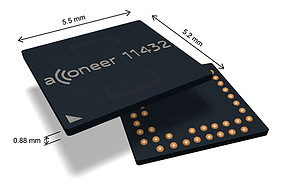
\includegraphics[scale=0.8]{figs_temp/acc_sensor}
	\caption{Image of the 60 GHz PCR radar sensor used in this work (retrieved from \url{www.acconeer.com/products} on 14/1/18).}
	\label{fig:acc_sens}
\end{figure}

\section{Objective}

In this work we, wish to explore whether it is possible to create an effective classification scheme from millimeter-wave radar response acquired during device movement. The classification task will be to accurately distinguish a grass surfaces from a selection of non-grass surfaces commonly found adjacent to lawns. All experiments will be performed using two 60 GHz pulsed coherent radar (\gls{pcr}) sensors from Acconeer, see Figure \ref{fig:acc_sens}, mounted at the front of device moving straight at a constant velocity. 

To this end, the Python programming language will be utilized together with Scikit learn and Keras with a TensorFlow backend for development \citep{scikit-learn}, \citep{chollet2015}, \citep{tensorflow2015-whitepaper}. 




%In this work, we seek to create a model capable of performing binary surface classification from data collected during robot movement. By collecting data on grass surfaces and selection of non-grass surfaces we wish to create an effective classifier able to distinguish a grass covered surface from other surface types. All experiments will be performed using two 60 GHz pulsed coherent radar (\gls{pcr}) sensors from Acconeer, see figure \ref{fig:acc_sens},  mounted on the front of device moving straight at a constant velocity. 

\section{Thesis Outline}

The outline of this thesis is as follows:
\\ \\
\noindent\textbf{Chapter 2:} This chapter explains the fundamentals of \gls{pcr} systems, and describes how distance, reflectivity and radial velocity can be extracted from the radar response. The method in which radar measurements are carried out is explained, as well as the \gls{iq} demodulation procedure.
\\ \\
\noindent\textbf{Chapter 3:} In chapter 3, we proceed with describing the data collection method. Sensor settings, such as pulse length and sampling frequency, are discussed. 
\\ \\
\noindent\textbf{Chapter 4:} Chapter 4 presents the feature extraction process. Temporal features, such as the autocovariance, are investigated for accurate surface classification. At the end of the chapter, one of the tested extraction methods is selected for further use. 
\\ \\
\noindent\textbf{Chapter 5:}  In this chapter, a few different classifiers are tested for prediction accuracy. A selection of two linear and four non-linear machine learning models are tested. At the end of the chapter, one machine learning classifier is selected as the most suitable. 
\\ \\
\noindent\textbf{Chapter 6:} In chapter 6, data augmentation and outlier suppression is discussed.  
\\ \\
\noindent\textbf{Chapter 7:} Chapter 7 examines the capabilities of the found model in real and artificially created test scenarios. The found results, as well as some error sources and limitations, are discussed.
\\ \\
\noindent\textbf{Chapter 8:} In chapter 8, conclusions of this work are presented and possible directions of future work are discussed. 





%In spite of their rise in populatity, solutions for surface classification using high frequency radars are somewhat scarce. When a single radar sensor is used for this purpose and a nonstationary setting is considered such as for a device moving across a surface of interest, very little previous work can be found in litterature. The perhaps closest resemblance is the RadarCat project\citep{yeo_2016}. As a part of Google's project Soli, RadarCat used a radar sensor for material classification. Nonetheless, a central part of this approach was having an object stationary and in direct contact with the radar sensor. The focal point of Project Soli was gesture recognition. This application bears some similarities to surface classification in motion in the regard that the subject is nonstationary. However classifying surfaces during motion and classifying hand gestures differ on a critical point - gestures are actions performed during some window in time while a robot moving along a surface is a continuous operation. 



%Continue: You want to be able to do this on a budget.


%\subsection{Previous work}


%It is in many applications of interest to obtain images of subsurface identification nondestructively. In recent decades, ground penetrating radar (GPR) has found increasing use in evaluation of road conditions \citep{solla_gonzález-jorge_varela_lorenzo_2013} for preservation and maintenance of infrastructure.


%A major challenge in radar sensing is to not only detect, but also to identify radar targets. This can for example be used for monitoring of urban environments \citep{harter_kowalewski_sit_jalilvand_ziroff_zwick_2014}.


%Localization is the classic use-case for radars. 
%\\ \\
% Radar  can detect relatively small targets at near or far distances and can measure their range with  precision  in  all weather,  which is  its chief  advantage when compared with other  sensors \citep{skolnik_2009}
%\\ \\
%Radar classification: 


% Classifying underground objects - this is a good paper we should look deeper into
%Using a ground penetrating radar (GPR), it is possible to identify subsurface objects. 
%Significantly lower frequency (900 MHz)
%\citep{lu_pu_liu_2014}.
% Paper on ground penetrating radar
%\citep{daniels_2004}

% RadarCat


%Chapter 3: Mention something about the data collecting process. Motive our choice of parameters such as sampling frequency. Go through visual observations of our data.

%Chapter 4: Feature selection and preprocessing is considered. Signal structure is discussed primarily on an intuitive level. 

%Chapter 5: Classification schemes. Moving from simple to advanced, some classifiers of special interest are investigated. Results with regards to these classifiers are presented.

%Chapter 6: Disucssion.

%Chapter 7: Conclusion.
